\documentclass[letterpaper,11pt]{report}

\usepackage{fullpage}
\usepackage{verbatim}
\usepackage{cite}
\usepackage{setspace}
\usepackage{fancyhdr}

\usepackage{textcomp}
\usepackage{bm}
\usepackage{mathtools}

%\usepackage{noReferences}
\usepackage[small]{caption}
\usepackage{graphics}
\usepackage{color}

\usepackage{hyperref}

%\usepackage{natbib}

\usepackage[dvips]{graphicx}
 % define the title

% Paper conservation layout. Long live the trees!!
\setlength{\oddsidemargin}{-0.4mm} % 25 mm left margin
\setlength{\evensidemargin}{\oddsidemargin}
\setlength{\textwidth}{160mm}      % 25 mm right margin
\setlength{\topmargin}{-5.4mm}     % 20 mm top margin
\setlength{\headheight}{5mm}
\setlength{\headsep}{5mm}
\setlength{\footskip}{10mm}
\setlength{\textheight}{237mm}     % 20 mm bottom margin


\setlength{\parskip}{1ex}
\parindent 0in
\def\SAONE{Specific Aim 1}
\def\SATWO{Specific Aim 2}
\def\SATHREE{Specific Aim 3}
\def\SAFOUR{Specific Aim 4}

\def\title{GPU assisted volume rendering with OptiX}

%\def\titletwo{Thesis Proposal Title Line 2}

\def\optix{Nvidia\textsuperscript{\textregistered} OptiX\texttrademark\ }
\def\cuda{CUDA\textsuperscript{\textregistered}\    }
\def\R{{\rm I\!R}}
\def\Rthree{{\rm I\!R^3}}
\def\Rfour{{\rm I\!R^4}}
\def\rxy{\bm{r_{xy}}}
\def\dt{\bm{\Delta t}}

\begin{document}



\def\addrone{Your address}
\def\addrtwo{Your city}

\def\degree{B.Tech. in Computer Science and Engineering}

\def\btptrack{Research}
 %add the track applicable
% current options: Research, Engineering, or Entrepreneurship

\def\submissiondate{November 17, 2016}

\def\supervisorone{Dr. Ojaswa Sharma (Thesis Advisor)}

\def\supervisortwo{Dr. Viswnath Gunturi (Internal Examiner)}
\def\supervisorthree{Dr. Ganga Bahubalindruni(Internal Examiner)}

%\def\supervisorfour{XXX XXXX }
%\def\supervisorfive{YYY YYYY}

\thispagestyle{empty}

\vspace{5.65in}

\begin{center}

\vspace{5.65in}

{\LARGE \bf {GPU ASSISTED VOLUME RENDERING WITH OptiX}

 }
 \vspace{.3in}

% \font{28pt}
 {\Large{Student Name: Sambhav Satija}} \\
 {\large{Roll Number: 2013085}} \\
 \vspace{.1in}

 %\font{20pt}
%IIIT-D-BTech-CSE-2009-001 \\


    \vspace{.65in}

%  \vspace{.25in}


\vspace{.65in}


 {BTP report submitted in partial fulfillment of the requirements
\\for the Degree of B.Tech. in Computer Science \& Engineering}

%\vspace{.65in}

on {17\textsuperscript{th} November, 2016} \\
 %\copyright 2011 SSSSSS SSSSSS \\ All rights reserved \\

\vspace{.65in}

\textbf{BTP Track}: \btptrack\\
\quad\\

  {\textbf{BTP Advisor} \\
\supervisorone              \\
\supervisortwo \\
\supervisorthree \\ }
%\supervisorfour \\
%\supervisorfive} \\
\vspace{3.0in}


{Indraprastha Institute of Information Technology\\
New Delhi}



\end{center}

%This research was partially funded by XXXX YYYY.



%\newpage
%
%\pagestyle{empty}
%\vspace*{7.1in}

\newpage

\begin{center}
\textbf{\Large Student's Declaration}\label{section:declaration}
\end{center}
%\vspace{3in}
I hereby declare that the work presented in the report entitled \textbf{``GPU assisted volume rendering with OptiX"} submitted by me for the partial fulfillment of the requirements for the degree of \emph{Bachelor of Technology} in \emph{Computer Science \& Engineering} at
 Indraprastha Institute of Information Technology, Delhi, is an authentic record of my work carried out under guidance of \textbf{Dr. Ojaswa Sharma}. Due acknowledgements have  been given in the report to all material used. This work has not been submitted anywhere else for the reward of any other degree.
 \\ \vspace{0.5in}

\textbf{..............................}\hfill
\textbf{New Delhi, 17\textsuperscript{th} November 2016} \\
\textbf{Sambhav Satija}\\


% \doublespacing


\vspace{3in}
%\iffalse
\begin{center}
\textbf{\Large Certificate} \label{section:certificate}
\end{center}
%\vspace{3in}
This is to certify that the above statement made by the candidate is correct to the best of my knowledge.
 \\ \vspace{0.4in}

\textbf{..............................}\hfill
\textbf{New Delhi, ........ November 2016} \\
\textbf{Dr. Ojaswa Sharma}\\



\pagebreak

\begin{abstract}
Algorithms for rendering volumes (which evaluate the Volume Rendering Integral to different extents), can be be transformed into their parallel versions with varying improvements in performance. GPUs (Graphics Processing Units) have improved a lot in the past few years, however rendering systems still need to be designed in a way so as to utilise GPUs efficiently. In this project, we explore the possibility of using \optix, a ray tracing framework by Nvidia to architect a fast volume rendering system.
  \\

\vspace{2in}
Keywords: Computer Graphics, Volume rendering, GPU, Nvidia OptiX
\end{abstract}

\newpage



\section*{Acknowledgments}\label{section:acknowledgments}
\pagestyle{plain}
\pagenumbering{roman}

I would like to thank Dr. Ojaswa Sharma for being a tremendously patient advisor. This project, until now, has been an incredible learning experience, which was possible only because of his guidance.
I am grateful to my family and friends for all their love and support.

\vspace{2in}
\section*{Work Distribution}
This is an independent project.

\newpage

\tableofcontents

%\newpage

%\newpage

% \newpage
% \mbox{}


%\doublespacing



\chapter{Introduction}\label{chapter:introduction}
%\pagestyle{fancy}
\pagenumbering{arabic}
\setcounter{page}{1}
\onehalfspacing

\section{Problem description}
There are a lot of sources of volumetric data (3D scalar fields), typically medical imaging diagnostic techniques such as CT/MRI scans or abstract mathematical data such as 3D probability distributions. There is a growing need to render these volumes beautifully and in realtime, which  to a more enriching experience for the viewer while trying to comprehend the information. \\
GPUs are extremely good at solving parallel algorithms, with limitations on how the algorithms can be designed for improving performance. We'll be using the raytracing middleware \optix to build a volume rendering system on top of it.

\section{Current solution}
Since GPU designers have opened platforms like \cuda for using GPUs as general purpose computing devices (termed GPGPUs), it has been extremely easy to port naive parallel algorithms. \optix provides the bare minimal framework for building raytracing solutions, which we'll be selectively using to push the computation for volume rendering to the GPU.

\section{Organisation of this report}
This report includes the work done in the first semester of this project. The goal was to use \optix to build a functional, dynamic and real time volume rendering system. The motiviation behind choosing \optix as the framework is covered in
chapter ,%todo
an analysis on \optix is done in and %todo
the system built is described in chapters %todo.




\chapter{Literature Prerequisites}

\section{Basic Terminology}
Volumetric data is usually in the form of 3D scalar fields, which can be extracted from medical imaging devices, 3D distribution functions and computational fluid dymanics. A volume data can be extracted from any signal $f$ where

\[ f(\bm{x}) \in \R\  and\  \bm{x} \in \Rthree \]


Readily available volume data is usually in the form of a dump of intensity value at each voxel in the volume. A voxel is the basic single unit of the representation of 3D space, analogous to a pixel in 2D space. Each intensity value can be thought of as belonging to different isosurfaces in the volume.

Direct Volume Rendering (DVR) methods, instead of extracting isosurface information, render the data by evaluating an optical model based on how the raw volume emits, scatters and absorbs light. In DVR, each intensity value is thus mapped to different colour and alpha values. This mapping function is typically termed as a \textbf{transfer function}, which can be a one-to-one mapping, a linear interpolation of colours and alpha values at control points, or any function in general.

\[ transfer(\bm{i}) \in  \Rfour\ and\  \bm{i} \in isovalues\ in\ dataset  \]

Image order algorithms render the data by iterating over the pixels in the image, instead of the voxels or isosurfaces in the volume data.


\section{Raymarching}
One of the widely used volume rendering techniques is the Raymarching method. Raymarching is an image-order algorithm which renders the image one pixel at a time and employs DVR. Raymarching emits rays for every pixel on the screen from the camera.

Each ray is denoted by $\rxy$ for every $\bm{x}$ , $\bm{y}$ in the screen. The ray $\rxy$ is parameterised by $\bm{t}$, where $\bm{t}$ is the distance of the point from the camera. A point $\bm{x}$ on $\rxy$ is given by
\[ \bm{x} = \bm{camera} + \bm{t} \cdot \bm{dir(\rxy)} \]

The ray $\rxy$ traverses through the volume data, updating its colour as it passes through different intensities and finally sets the pixel $\bm{x}$, $\bm{y}$ to the composited colour. The ray $\rxy$ traverses the volume by stepping through the it with a fixed \textbf{stepping distance}, $\dt$. A lookup on the volume data returns the intensity at that point $\bm{x(t)}$. A transfer function maps this intensity value to a colour and alpha value. \\

This method of accumulation of colour using the alpha values is termed as \textbf{alpha blending} and be solved using 2 approaches:

\begin{itemize}
    \item \textbf{Front to back:\ }
        In this technique, the ray is traversed in the front to back manner; with $\bm{i}: (n-1) \xrightarrow[]{} 0$. $\bm{C^\prime_0}$ is the final colour of the pixel.

        \[ C^\prime_i = C_i + (1 - A_i)C^\prime_{i+1} \ \ \  where\ C^\prime_n = 0 \]

    \item \textbf{Back to front:\ }
        In this technique, the ray is traversed in the back to front direction; with $\bm{i}: 1 \xrightarrow[]{} n$.  $\bm{C^\prime_n}$ is the final colour of the pixel.

        \[ C^\prime_i = C^\prime_{i-1} + (1 - A^\prime_{i-1}) \cdot C_i \ \ \ where\ C^\prime_0 = 0 \]
        \[ A^\prime_i = A^\prime_{i-1} + (1 - A^\prime_{i-1}) \cdot A_i \ \ \ where\ A^\prime_0 = 0 \]
\\


    In both the above methods, $\bm{n} = \frac{\bm{exit(\rxy)} - \bm{enter(\rxy)}}{\dt}$,
        $\bm{enter(\rxy)}$ returns the point $\bm{x}$, the point where $\rxy$ enters the volume and
        $\bm{exit(\rxy)}$ returns the point $\bm{x}$, the point where $\rxy$ exits the volume.

    \newpage

    $\bm{C_i}$ and $\bm{A_i}$ are the colour and alpha values returned after two texture lookups. The first lookup returns the intensity value at point $\bm{i}$ on $\rxy$. The second lookup gives the colour and alpha for this intensity value. \newline

    Front to back compositing has a major optimisation that it can terminate early, as soon as the alpha crosses 1. However, this usually leads to decreased performance in GPUs due to processors in a warp running in lockstep. So back to front compositing is usually implemented.

\end{itemize}




\chapter{System Overview}

This chapter is split into 3 section. The first section gives a broad overview of the architecture. The second section gives a walkthrough of the system. The third section gives an overview on how the project evolved.

\section{Architecture overview}

\begin{figure}[h!]
 \centering
  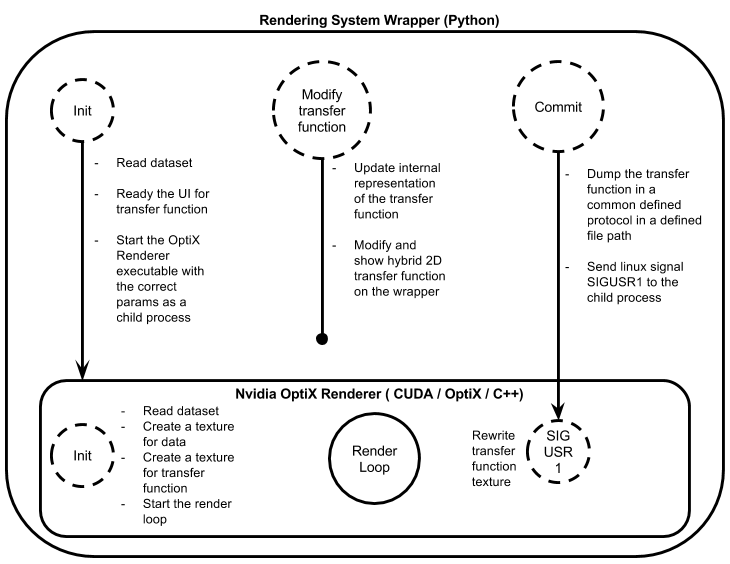
\includegraphics[width=0.95\textwidth]{arch1.png}
  \caption{System Architecture.}
  \label{fig:arch1}
 \end{figure}

Figure \ref{fig:arch1} shows the architecture of the system designed. The volume rendering computation is done in an binary executable written in C++ on top of the \optix platform. A Python wrapper is written for convenience which allows the user to dynamically create and update the transfer functions.\

This transfer function can be pushed to the executable dynamically. The rendering executable maps the transfer function texture to the device at runtime again, showing immediate results. The rendering binary interops between OpenGL to display the rendered buffer on-screen.

\section{Working}
This section describes a sample workflow of the program.

\begin{enumerate}
    \item
    Starting the python script starts the wrapper program, which asks for the volume data file \ref{fig:working1}. The current project can understand NRHD data file formats.

    \begin{figure}[h!]
     \centering
      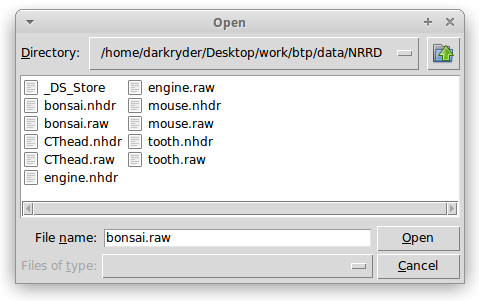
\includegraphics[width=0.4\textwidth]{working1.png}
      \caption{Prompt for datafile.}
      \label{fig:working1}
     \end{figure}

    \item
    The wrapper shows a transfer function editing screen \ref{fig:working2} that allows the user to modify the transfer function.

    A histogram of the isovalues in the dataset is the background of the transfer function editor. This can act as a help to the user for selecting good control points.

    \begin{figure}[h!]
     \centering
      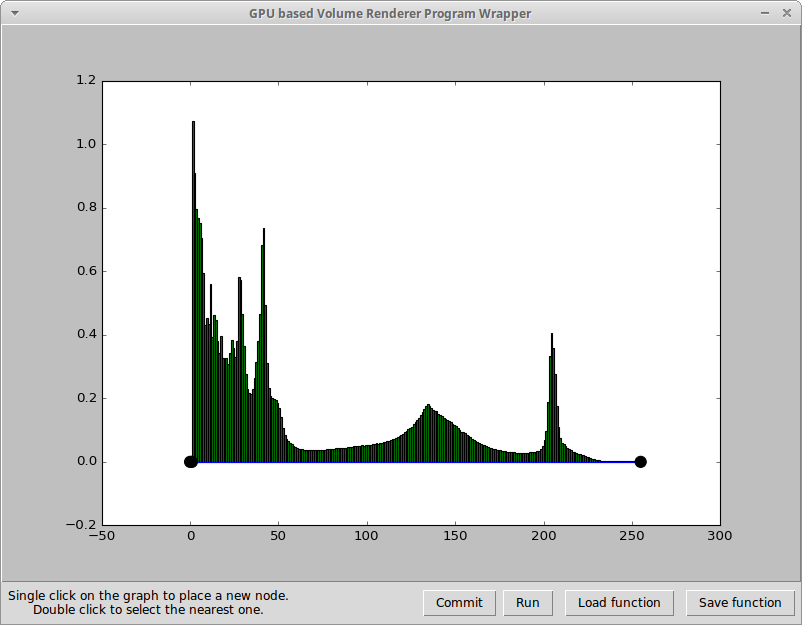
\includegraphics[width=0.4\textwidth]{working2.png}
      \caption{Transfer function editor.}
      \label{fig:working2}
     \end{figure}

    \item
    Clicking anywhere on the graph editor adds a control point to that isovalue/alpha graph. The color for that control node can be selected from the prompt \ref{fig:working3}.

    \begin{figure}[h!]
     \centering
      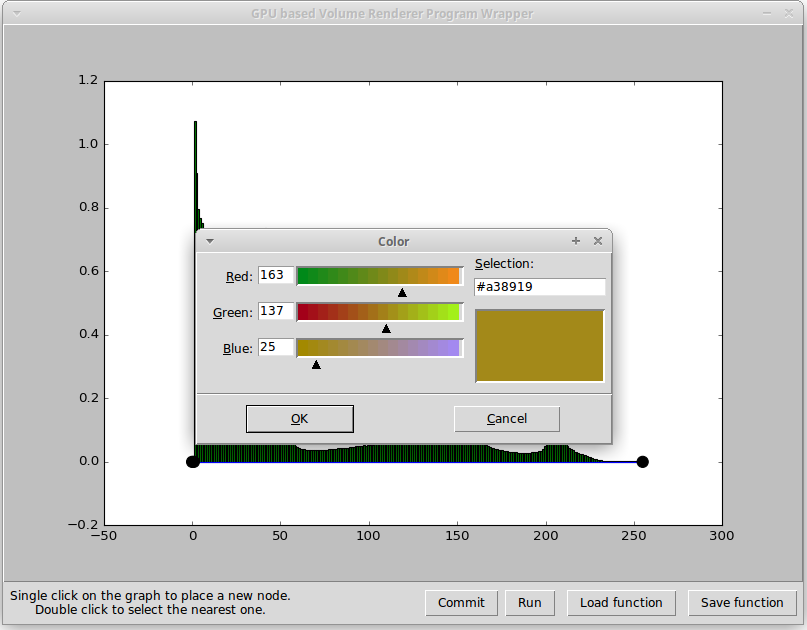
\includegraphics[width=0.4\textwidth]{working3.png}
      \caption{Selecting a color for control node.}
      \label{fig:working3}
     \end{figure}

    \item
    This allows creating simple transfer functions extremely fast. The transfer function does linear interpolation for the alpha value and color for any isovalue for which the values are not explicitly defined. \ref{fig:working4}.

    \begin{figure}[h!]
     \centering
      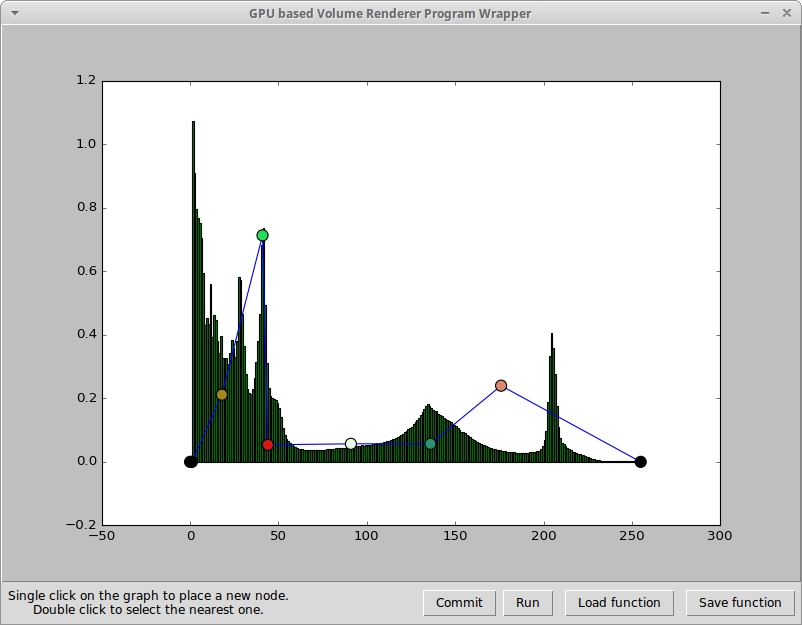
\includegraphics[width=0.4\textwidth]{working4.png}
      \caption{Fast creation of control points in nodes.}
      \label{fig:working4}
     \end{figure}

     \item
     Clicking on \textbf{Run} starts the rendering executable as a child process of the wrapper with the corresponding required arguments. \ref{fig:working5}.

    \begin{figure}[h!]
     \centering
      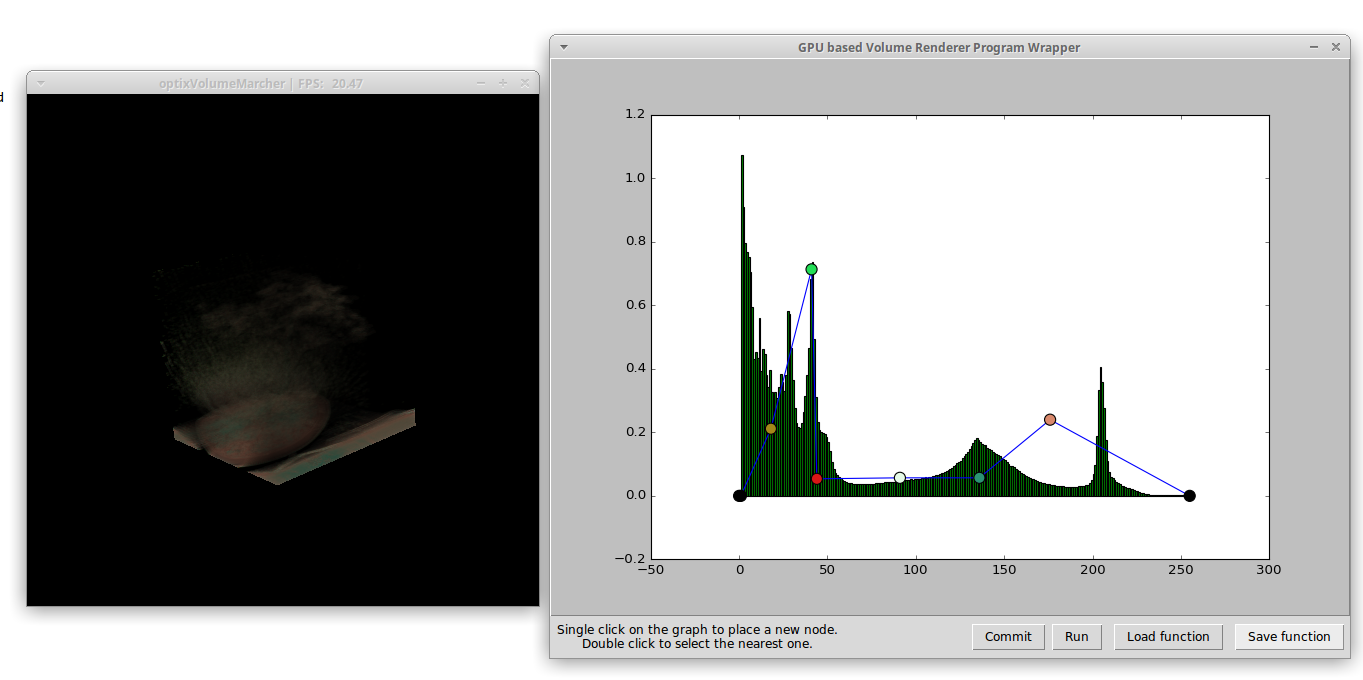
\includegraphics[width=0.4\textwidth]{working5.png}
      \caption{Booting up the rendering system.}
      \label{fig:working5}
     \end{figure}

\newpage

     \item
     Already added nodes can be intuitively modified/deleted by double clicking and moving them around in the editor. Simply clicking the \textbf{Commit} button will send this modified transfer function to the rendering process.\\
     The rendering executable dynamically reloads the transfer function texture to the device and the new results are instantly visible. \ref{fig:working6}

    \begin{figure}[h!]
     \centering
      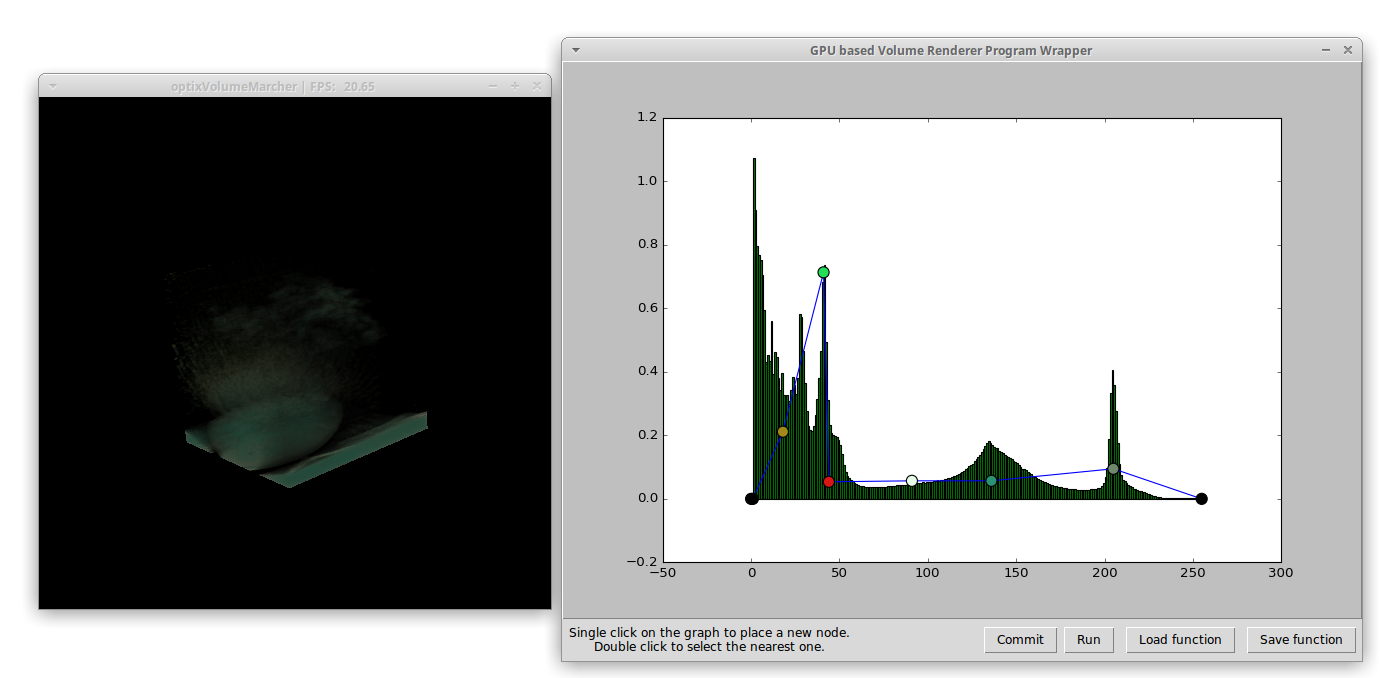
\includegraphics[width=0.4\textwidth]{working6.png}
      \caption{Instant update of transfer function.}
      \label{fig:working6}
     \end{figure}

      \item
    Convenience features like loading and saving transfer functions are also present \ref{fig:working7}.

    \begin{figure}[h!]
     \centering
      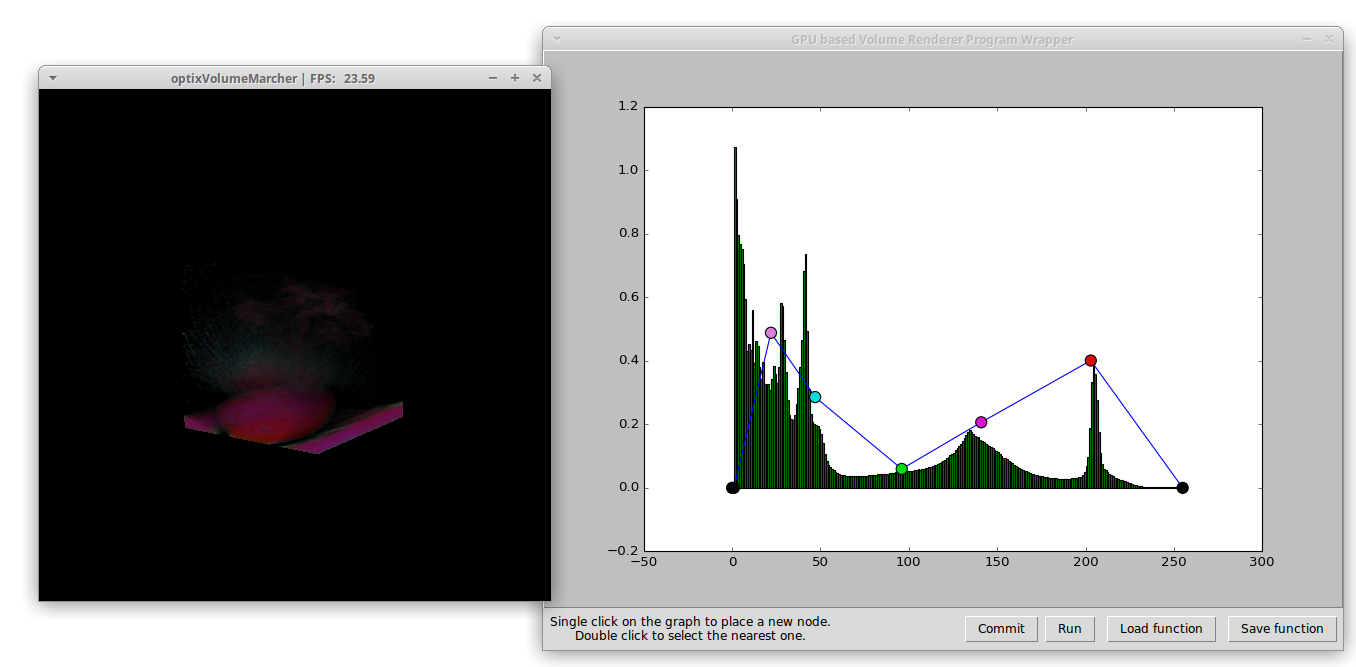
\includegraphics[width=0.4\textwidth]{working7.png}
      \caption{A transfer function loaded from a previous session and auto reloaded into the executable.}
      \label{fig:working7}
     \end{figure}

\end{enumerate}

\section{Progress Report}

    \begin{figure}[h!]
     \centering
      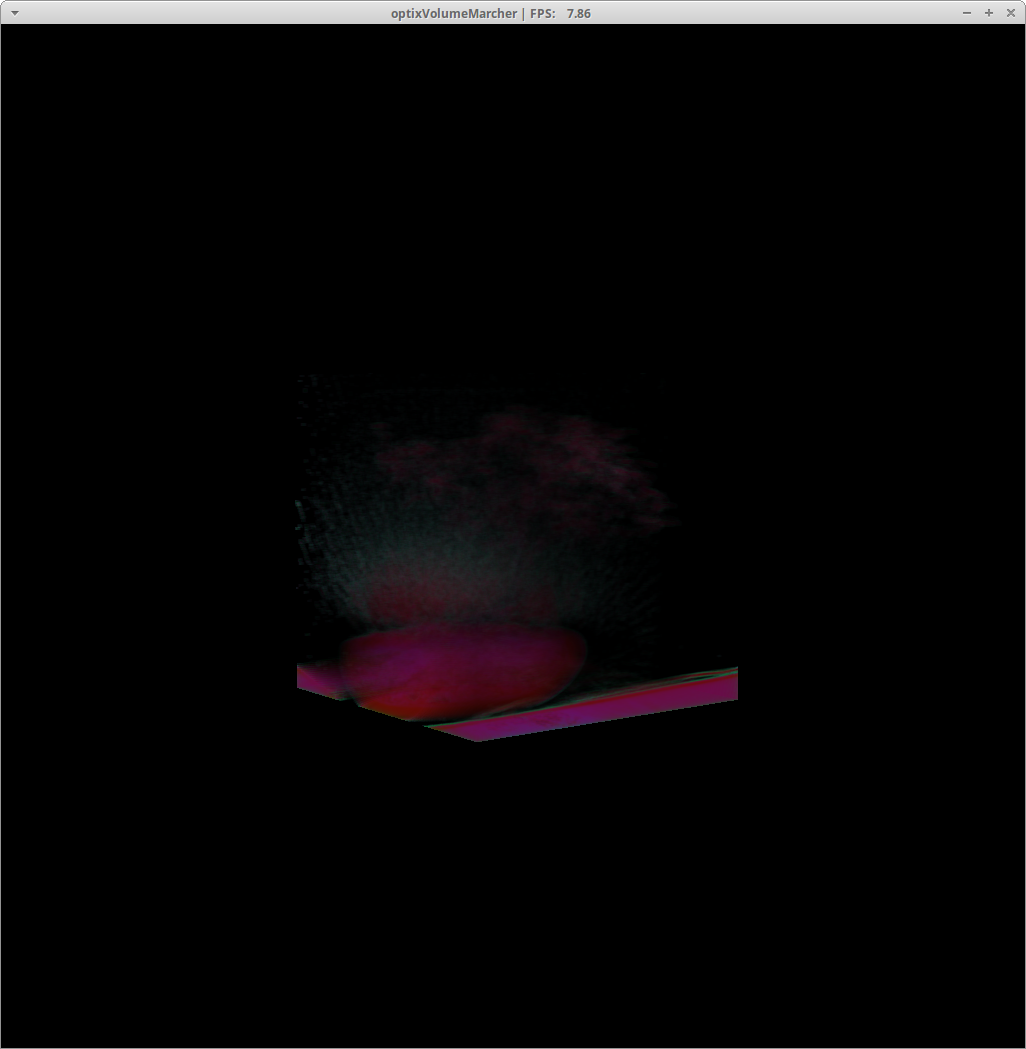
\includegraphics[width=0.8\textwidth]{working8.png}
      \caption{Scene from rendering executable.}
      \label{fig:working8}
     \end{figure}






\chapter{Discussion}

\chapter{Appendix: Evaluating \optix}

% \cite{Perugini:2007:SOI:1240624.1240770}


%\newpage
%\bibliographystyle{these}
\bibliographystyle{acm}
%\bibliographystyle{elsart-harv}
%\newpage
%\section{References}
%\bibliography{Library}
\bibliography{sample}

%\chapter*{Appendix}\label{chapter:appendix}

\end{document}
